\chapter{Calculer un $Q$ pour un $T_\text{retour}$ donné -- \textit{Séries annuelles}}

\fbox{ %fbox est utilisé pour voir les bords de la minipage
    \begin{minipage}[l]{17cm}
        L'étude et la marche à suivre conviennent pour des séries statistiques avec un débit maximal annuel ! \\
        Cela veut dire que pour chaque année (et chaque mois) nous avons le débit maximal, le tout sur une période donnée (plusieurs années) (ex. Tab. \ref{tab:serieAnnuelleMaximum})
    \end{minipage}
}

Nous avons les données suivantes :
\begin{table}[H]
    \centering
    \begin{tabular}{|c||c|c|c|c|c|c|c|c|c|c|c|c|}
        \hline
        \textbf{Année} & \textbf{Jan} & \textbf{Fev} & \textbf{Mar} & \textbf{Avr} & \textbf{Mai} & \textbf{Juin} & \textbf{Jui} & \textbf{Aoû} & \textbf{Sep} & \textbf{Oct} & \textbf{Nov} & \textbf{Dec} \\
        \hline \hline
        \textbf{1965}  & 11 & \cellcolor{green}10 & 14 & 15 & 160 & 205 & 205 & \cellcolor{red}350 & 145 &  84 &  21 & 18 \\
        \hline
        \textbf{1966}  & \cellcolor{green}17 & 19 & 17 & 47 & 105 & \cellcolor{red}175 & 155 & 150 &  97 & 125 &  25 & 20 \\
        \hline
        \textbf{\dots} &    &    &    &    &     &     &     &     &       &     &     &      \\
        \hline
        \textbf{1992}  & 14 & \cellcolor{green}13 & 17 & 62 & 110 & \cellcolor{red}290 & 225 & 215 & 175 &  75 &  46 & 38 \\
        \hline
        \textbf{1993}  & 28 & 42 & 38 & 49 & 125 & 200 & 180 & 150 & \cellcolor{red}460 & 170 &  37 & \cellcolor{green}27 \\
        \hline
    \end{tabular}
    \caption{Tableau avec les débits maximums pour chaque mois entre les années 1965 et 1993}
    \label{tab:seriesAnnuellesMaximum}
\end{table}


\section{Contrôler la stationnarité}
Le contrôle de la stationnarité se fait en créant le graphique des débits maximales par années (cf. Figure \ref{graph:stationnarite})
\begin{figure}[H]
    \centering
    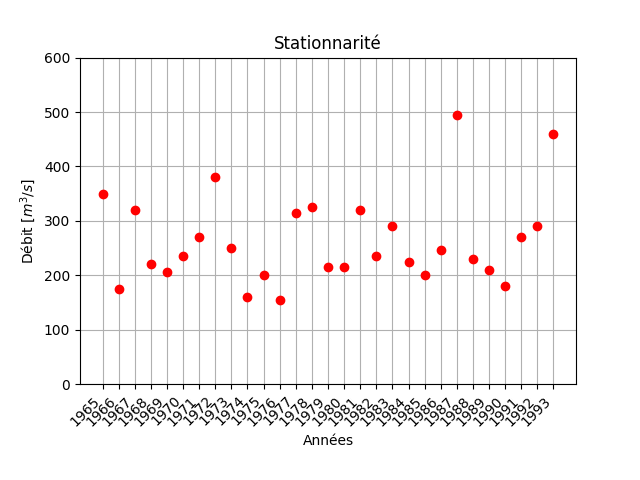
\includegraphics[width=12cm]{stationnarite.png}
    \caption{Stationnarité (étude entre 1965 et 1993)}
    \label{graph:stationnarite}
\end{figure}


\section{Contrôler l'homogénéité -- \textit{Optionnel}}
Afin de contrôler l'homogénéité des débits, il faut tracer un graphique avec les débits maximums mensuels et pour toutes les années (cf. Figure \ref{graph:homogeneite}).
\begin{figure}[H]
    \centering
    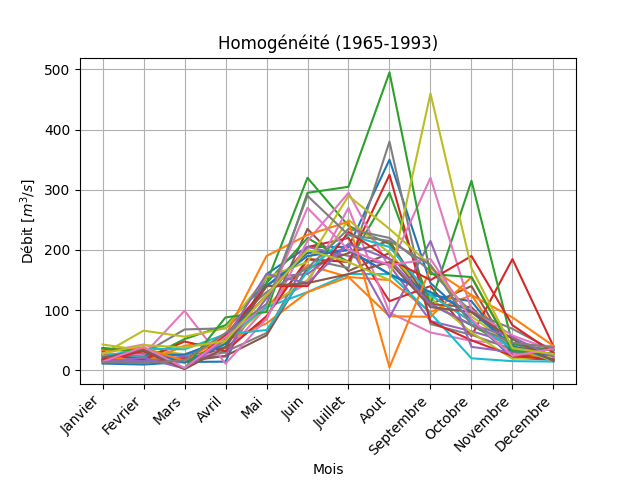
\includegraphics[width=12cm]{homogeneite.png}
    \caption{Homogénéité (étude entre 1965 et 1993)}
    \label{graph:homogeneite}
\end{figure}


\section{Calcul des temps de retour $T$}
\begin{enumerate}
    \item Garder les débits maximums annuels
    \item Classer les débits par ordre croissants
    \item Inscrire le rang pour chaque débit
    \item Calculer le temps de retour selon la formule choisie (cf. \ref{tab:formuleTempsRetour}) \\
    \underline{Conseil :} utiliser la \textbf{{\color{red} formule de Hazen}} et utiliser une autre formule pour comparer
\end{enumerate}



\section{Calcul des paramètres de la loi de Gumbel} \label{sec:parametreLoiGumbel}
\begin{enumerate}
    \item Calcul de la fonction $F(Q_\text{obs})$ pour chaque débit \formule{5}{\ref{tab:loiGumbel}} ;
    \item Calcul des divers paramètres de la série statistique :
    \begin{itemize}
        \item Moyenne des débits observés ; \\
        \excel{=MOYENNE()}
        \item Ecart-type de la moyenne des débits observés ; \\
        \excel{=ECARTYPE.STANDARD()}
        \item Paramètre $a$ \formule{3}{\ref{tab:loiGumbel}}
        \item Paramètre $b$ \formule{4}{\ref{tab:loiGumbel}}
    \end{itemize}
    \item Calcul du débit Gumbel pour chaque temps de retour
    \begin{enumerate}
        \item Paramètre $U$ \formule{8}{\ref{tab:loiGumbel}}
        \item Débit $Q_\text{Gumbel}$ \formule{7}{\ref{tab:loiGumbel}}
    \end{enumerate}
    \item Créer les graphiques suivants \\
    \begin{tabular}{lll}
        \toprule
                                    & \textbf{Variable réduite $U$} & \textbf{Débit selon la loi de Gumbel} \\
        \midrule
        \multirow{2}{*}{Abscisse}   & Variable réduite $U$ [-]      & Temps [années]                        \\
                                    &                               & Échelle logarithmique                 \\            
        Ordonnée                    & Débit [\ms]                   & Débit [\ms]                           \\
        \midrule
        Courbes :                   & ...                           & ...                                   \\
        \midrule
        Références                  & Figure X                      & Figure X                              \\
        \bottomrule
    \end{tabular}
\end{enumerate}

\section{Extrapolation d'un débit en fonction du temps de retour}
\begin{enumerate}
    \item Poser les temps de retour rares que vous souhaitez
    \item Procédez à l'étape 3 du paragraphe \ref{sec:parametreLoiGumbel}
    \item Ajoutez la courbe sur les graphiques X et X
\end{enumerate}
